\documentclass{article}
\usepackage[utf8]{inputenc}
\usepackage[paperwidth=3.25in,paperheight=1.75in,margin=0in]{geometry}
\usepackage{tikz}
\usepackage{amsmath,amssymb}
\usepackage{xcolor}

\begin{document}
\pagestyle{empty}
\noindent
% Dimensions strictly 3.25 in x 1.75 in (8.25 cm x 4.45 cm)
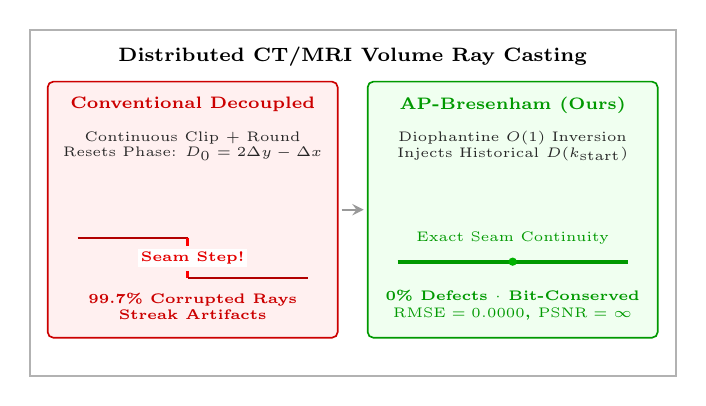
\begin{tikzpicture}[x=1in, y=1in]
    % Bounding box to enforce exactly 3.25in x 1.75in
    \clip (0, 0) rectangle (3.25, 1.75);
    \fill[white] (0, 0) rectangle (3.25, 1.75);
    \draw[gray!60, line width=0.75pt] (0.01, 0.01) rectangle (3.24, 1.74);

    % Title header
    \node[anchor=north, font=\fontsize{7}{8}\selectfont\bfseries, text=black] at (1.625, 1.70) 
        {Distributed CT/MRI Volume Ray Casting};

    % Left Box: Conventional
    \draw[red!80!black, fill=red!6, rounded corners=2pt, line width=0.6pt] (0.1, 0.20) rectangle (1.55, 1.48);
    \node[anchor=north, font=\fontsize{6}{7}\selectfont\bfseries, text=red!80!black] at (0.825, 1.45) 
        {Conventional Decoupled};
    \node[anchor=north, font=\fontsize{4.8}{5.5}\selectfont, text=black!85, align=center] at (0.825, 1.28) 
        {Continuous Clip + Round\\Resets Phase: $D_0=2\Delta y - \Delta x$};
    
    % Seam artifact icon (broken line)
    \draw[thick, red!70!black] (0.25, 0.70) -- (0.8, 0.70);
    \draw[dashed, red, line width=1pt] (0.8, 0.70) -- (0.8, 0.50);
    \draw[thick, red!70!black] (0.8, 0.50) -- (1.4, 0.50);
    \node[font=\fontsize{5}{6}\selectfont\bfseries, text=red!90!black, fill=white, inner sep=1pt] at (0.825, 0.60) {Seam Step!};
    
    \node[anchor=south, font=\fontsize{5}{6}\selectfont\bfseries, text=red!80!black, align=center] at (0.825, 0.24) 
        {99.7\% Corrupted Rays\\Streak Artifacts};

    % Right Box: AP-Bresenham
    \draw[green!60!black, fill=green!6, rounded corners=2pt, line width=0.6pt] (1.70, 0.20) rectangle (3.15, 1.48);
    \node[anchor=north, font=\fontsize{6}{7}\selectfont\bfseries, text=green!60!black] at (2.425, 1.45) 
        {AP-Bresenham (Ours)};
    \node[anchor=north, font=\fontsize{4.8}{5.5}\selectfont, text=black!85, align=center] at (2.425, 1.28) 
        {Diophantine $O(1)$ Inversion\\Injects Historical $D(k_{\mathrm{start}})$};
    
    % Continuous smooth line
    \draw[line width=1.4pt, green!60!black] (1.85, 0.58) -- (3.00, 0.58);
    \fill[green!70!black] (2.425, 0.58) circle (1.5pt);
    \node[anchor=south, font=\fontsize{4.8}{5.5}\selectfont, text=green!60!black] at (2.425, 0.62) {Exact Seam Continuity};

    \node[anchor=south, font=\fontsize{5}{6}\selectfont\bfseries, text=green!60!black, align=center] at (2.425, 0.24) 
        {0\% Defects $\cdot$ Bit-Conserved\\$\mathrm{RMSE}=0.0000$, $\mathrm{PSNR}=\infty$};

    % Center divider arrow
    \draw[->, >=stealth, line width=0.8pt, gray!80] (1.57, 0.84) -- (1.68, 0.84);
\end{tikzpicture}
\end{document}
